\documentclass[12pt,a4paper]{article}

% ─── Page Layout ───────────────────────────────────────────────────────────────
\usepackage[a4paper, margin=0.8in, headheight=14pt]{geometry}

% ─── Fonts (XeLaTeX) ───────────────────────────────────────────────────────────
\usepackage{fontspec}
\usepackage{unicode-math}
\setmainfont{TeX Gyre Pagella}
\setmonofont[Scale=0.88]{TeX Gyre Cursor}
\setmathfont{Latin Modern Math}

% ─── Packages ──────────────────────────────────────────────────────────────────
\usepackage{xcolor}
\usepackage{colortbl}
\usepackage{titlesec}
\usepackage{enumitem}
\usepackage{tabularx}
\usepackage{booktabs}
\usepackage{array}
\usepackage{amsmath}
\usepackage{tikz}
\usetikzlibrary{shapes.geometric, arrows.meta, positioning, calc, fit, decorations.pathreplacing}
\usepackage{tcolorbox}
\tcbuselibrary{skins, breakable}
\usepackage{hyperref}
\usepackage{fancyhdr}
\usepackage{graphicx}
\usepackage{microtype}
\hyphenpenalty=10000
\exhyphenpenalty=10000
\sloppy
\usepackage{caption}
\usepackage{setspace}
\usepackage{multirow}
\usepackage{tocloft}

% ─── Q&A helper ────────────────────────────────────────────────────────────────
\newcommand{\Q}[1]{\textbf{#1}\par\noindent\ignorespaces}

% ─── Colour Palette ────────────────────────────────────────────────────────────
\definecolor{myred}{RGB}{196,30,58}
\definecolor{mydark}{RGB}{30,30,50}
\definecolor{mygreen}{RGB}{14,120,80}
\definecolor{myteal}{RGB}{0,130,140}
\definecolor{myamber}{RGB}{180,100,0}
\definecolor{mypurple}{RGB}{100,30,160}
\definecolor{mygray}{RGB}{246,247,249}
\definecolor{mgframe}{RGB}{180,185,200}
\definecolor{watermark}{RGB}{145,150,170}
\definecolor{hdrred}{RGB}{250,232,235}
\definecolor{hdrgreen}{RGB}{220,244,233}
\definecolor{hdrteal}{RGB}{220,242,244}
\definecolor{hdramber}{RGB}{253,242,215}
\definecolor{hdrpurple}{RGB}{238,228,255}
\definecolor{hdrgray}{RGB}{238,240,245}
\definecolor{rowalt}{RGB}{250,251,253}

% ─── Section Formatting ────────────────────────────────────────────────────────
\titleformat{\section}
  {\large\bfseries\color{myred}}{\thesection.}{0.5em}{}
  [\vspace{1pt}{\color{myred}\rule{\linewidth}{0.8pt}}]
\titleformat{\subsection}
  {\normalsize\bfseries\color{myteal}}{\thesubsection}{0.5em}{}
\titlespacing*{\section}{0pt}{18pt}{7pt}
\titlespacing*{\subsection}{0pt}{11pt}{4pt}

% ─── Paragraph ─────────────────────────────────────────────────────────────────
\setlength{\parindent}{0pt}
\setlength{\parskip}{4pt}

% ─── TOC Styling ───────────────────────────────────────────────────────────────
\renewcommand{\cfttoctitlefont}{\large\bfseries\color{myred}}
\renewcommand{\cftaftertoctitle}{\par\noindent{\color{myred}\rule{\linewidth}{0.8pt}}}
\setlength{\cftbeforetoctitleskip}{0pt}
\setlength{\cftaftertoctitleskip}{6pt}
\renewcommand{\cftsecfont}{\normalsize\bfseries\color{mydark}}
\renewcommand{\cftsecpagefont}{\normalsize\bfseries\color{mydark}}
\renewcommand{\cftsecleader}{\cftdotfill{\cftdotsep}}
\setlength{\cftbeforesecskip}{7pt}
\renewcommand{\cftsubsecfont}{\small\color{mydark}}
\renewcommand{\cftsubsecpagefont}{\small\color{mydark}}
\setlength{\cftbeforesubsecskip}{3pt}
\setlength{\cftsubsecindent}{1.4em}

% ─── Table helpers ─────────────────────────────────────────────────────────────
\renewcommand{\arraystretch}{1.45}
\setlength{\tabcolsep}{6pt}
\arrayrulecolor{mydark}
\newcolumntype{B}[1]{>{\small\bfseries\raggedright\arraybackslash}m{#1}}
\newcolumntype{Y}{>{\small\raggedright\arraybackslash}X}
\renewcommand{\tabularxcolumn}[1]{m{#1}}

% ─── Header / Footer ───────────────────────────────────────────────────────────
\pagestyle{fancy}
\fancyhf{}
\fancyhead[L]{\small\color{myred}\textbf{OE-EC604B}\;\color{mydark}--- Operating System}
\fancyhead[R]{\small\color{myteal}\textbf{Module 5 Notes}}
\fancyfoot[C]{\small\color{mydark}\thepage}
\fancyfoot[R]{\small\color{watermark}\textit{\copyright\ Biraj}}
\renewcommand{\headrulewidth}{0.5pt}
\renewcommand{\footrulewidth}{0.3pt}

% ─── Hyperref ──────────────────────────────────────────────────────────────────
\hypersetup{
  colorlinks=true, linkcolor=myteal, urlcolor=myteal,
  pdfauthor={Biraj Sarkar},
  pdftitle={OE-EC604B --- Module 5 Notes}
}

% ─── tcolorbox styles ──────────────────────────────────────────────────────────
\tcbset{
  tikzbox/.style={
    colback=mygray, colframe=mgframe, boxrule=0.6pt, arc=4pt,
    left=8pt, right=8pt, top=6pt, bottom=6pt,
    colbacktitle=mgframe, coltitle=mydark,
    fonttitle=\small\bfseries
  },
  defbox/.style={
    colback=hdrgreen, colframe=mygreen, boxrule=0.8pt, arc=4pt,
    left=9pt, right=9pt, top=6pt, bottom=6pt,
    colbacktitle=mygreen, coltitle=white,
    fonttitle=\small\bfseries
  },
  formulabox/.style={
    colback=hdrteal, colframe=myteal, boxrule=0.8pt, arc=4pt,
    left=9pt, right=9pt, top=7pt, bottom=7pt,
    colbacktitle=myteal, coltitle=white,
    fonttitle=\small\bfseries
  },
  examplebox/.style={
    colback=hdramber, colframe=myamber, boxrule=0.8pt, arc=4pt,
    left=9pt, right=9pt, top=6pt, bottom=6pt,
    colbacktitle=myamber, coltitle=white,
    fonttitle=\small\bfseries
  },
  masonbox/.style={
    colback=hdrpurple, colframe=mypurple, boxrule=0.8pt, arc=4pt,
    left=9pt, right=9pt, top=6pt, bottom=6pt,
    colbacktitle=mypurple, coltitle=white,
    fonttitle=\small\bfseries
  },
  exambox/.style={
    colback=hdrpurple, colframe=mypurple, boxrule=1pt, arc=5pt,
    left=10pt, right=10pt, top=8pt, bottom=8pt,
    colbacktitle=mypurple, coltitle=white,
    fonttitle=\bfseries,
    breakable, title after break={\textbf{Frequently Asked / Viva Questions (contd.)}}}
}
% Make all boxes breakable across pages
\tcbset{breakable}

% ─── TikZ styles ───────────────────────────────────────────────────────────────
\tikzset{
  block/.style={rectangle, draw=myteal, fill=hdrteal,
    text width=2.4cm, align=center, minimum height=0.95cm,
    font=\small, rounded corners=3pt, line width=0.7pt},
  redblock/.style={rectangle, draw=myred, fill=hdrred,
    text width=2.4cm, align=center, minimum height=0.95cm,
    font=\small, rounded corners=3pt, line width=0.7pt},
  greenblock/.style={rectangle, draw=mygreen, fill=hdrgreen,
    text width=2.4cm, align=center, minimum height=0.95cm,
    font=\small, rounded corners=3pt, line width=0.7pt},
  amberblock/.style={rectangle, draw=myamber, fill=hdramber,
    text width=2.4cm, align=center, minimum height=0.95cm,
    font=\small, rounded corners=3pt, line width=0.7pt},
  purpblock/.style={rectangle, draw=mypurple, fill=hdrpurple,
    text width=2.4cm, align=center, minimum height=0.95cm,
    font=\small, rounded corners=3pt, line width=0.7pt},
  sumjunc/.style={circle, draw=myamber, fill=hdramber,
    minimum size=0.62cm, font=\small, line width=0.8pt},
  arrow/.style={-Stealth, thick, color=mydark},
  redarrow/.style={-Stealth, thick, color=myred},
  line/.style={thick, color=mydark}
}

% ═══════════════════════════════════════════════════════════════════════════════
\begin{document}
% ═══════════════════════════════════════════════════════════════════════════════

\begin{center}
  {\LARGE\bfseries\color{myred} OE-EC604B --- Operating System}\\[5pt]
  {\normalsize\color{mydark} Semester VI \quad$\bullet$\quad 3L:0T:0P \quad$\bullet$\quad 3 Credits}\\[3pt]
  {\normalsize\color{myteal}\textbf{Module 5 Exam Notes: Deadlocks}}\\[3pt]
  {\small\color{mydark} CGEC \;$|$\; B.Tech ECE (2023--27) \;$|$\; \textit{Biraj Sarkar}}
\end{center}
\vspace{2pt}
\noindent{\color{myred}\rule{\linewidth}{1.5pt}}
\vspace{2pt}

\hypersetup{linkcolor=mydark}
\tableofcontents
\hypersetup{linkcolor=myteal}
\newpage

% ===============================================================================
\section{System Model and Deadlock Characterization}
% ===============================================================================

A \textbf{deadlock} is a state where a set of processes are blocked because each process is holding a resource and waiting for another resource held by some other process in the set.

\subsection{Four Necessary Conditions (Coffman Conditions)}
A deadlock situation can arise if and only if all four of the following conditions hold simultaneously in a system:
1. \textbf{Mutual Exclusion:} At least one resource must be held in a non-shareable mode (only one process can use it at a time).
2. \textbf{Hold and Wait:} A process must be holding at least one resource and waiting to acquire additional resources that are currently being held by other processes.
3. \textbf{No Preemption:} Resources cannot be preempted; a resource can be released only voluntarily by the process holding it, after that process has finished its task.
4. \textbf{Circular Wait:} A closed loop of processes must exist, where each process waits for a resource held by the next process in the loop. E.g., $P_0$ waits for $R_1$ (held by $P_1$), $P_1$ waits for $R_2$ (held by $P_2$), and $P_n$ waits for $R_0$ (held by $P_0$).

\subsection{Resource Allocation Graph (RAG)}
Deadlocks can be described precisely using a directed graph called a \textbf{Resource Allocation Graph (RAG)}:
\begin{itemize}[leftmargin=*, itemsep=3pt]
  \item \textbf{Vertices ($V$):} Divided into two partitions:
  \begin{itemize}[leftmargin=*, itemsep=2.5pt, topsep=0pt]
    \item Processes $P = \{P_1, P_2, \dots, P_n\}$ (represented by circles).
    \item Resource types $R = \{R_1, R_2, \dots, R_m\}$ (represented by rectangles containing dots for instances).
  \end{itemize}
  \item \textbf{Edges ($E$):}
  \begin{itemize}[leftmargin=*, itemsep=2.5pt, topsep=0pt]
    \item \textbf{Request Edge:} Directed edge $P_i \to R_j$ (process $P_i$ has requested resource $R_j$).
    \item \textbf{Assignment Edge:} Directed edge $R_j \to P_i$ (resource instance in $R_j$ is allocated to process $P_i$).
    \end{itemize}
  \end{itemize}

\begin{itemize}[leftmargin=*, itemsep=3pt]
  \item \textbf{Theorem:}
  \begin{itemize}[leftmargin=*, itemsep=2.5pt, topsep=0pt]
    \item If the RAG contains no cycles $\to$ No deadlock.
    \item If the RAG contains a cycle $\to$
      \item If single instance per resource type: Deadlock exists (cycle is necessary and sufficient).
      \item If multiple instances per resource type: Deadlock \textit{may} exist (cycle is necessary but not sufficient).
    \end{itemize}
  \end{itemize}

% ===============================================================================
\section{Deadlock Handling Strategies}
% ===============================================================================

Operating systems use three main strategies to handle deadlocks:

\subsection{1. Deadlock Prevention}
Ensures that the system can never enter a deadlock state by designing the system such that at least one of the four Coffman conditions cannot hold:
\begin{itemize}[leftmargin=*, itemsep=3pt]
  \item \textbf{Prevent Mutual Exclusion:} Make resources shareable (e.g., read-only files). \textbf{Drawback:} Some resources (printers, mutexes) are inherently non-shareable.
  \item \textbf{Prevent Hold and Wait:} Require processes to request all resources at once before execution, or release current resources before requesting new ones. \textbf{Drawback:} Low resource utilization; starvation.
  \item \textbf{Prevent No Preemption:} If a process holding resources requests another that cannot be immediately allocated, all its current resources are preempted (released). \textbf{Drawback:} Overhead of saving/restoring process states.
  \item \textbf{Prevent Circular Wait:} Impose a global ordering on all resource types (e.g., $F(R_j) = i$) and require processes to request resources only in strictly increasing order of enumeration. \textbf{Advantage:} Most practical prevention strategy.
\end{itemize}

\subsection{2. Deadlock Avoidance}
Requires that the OS has prior knowledge of the maximum resources a process will ever request.

\begin{tcolorbox}[defbox, title={\textbf{Safe State vs Unsafe State}}]
A state is \textbf{safe} if there exists a \textbf{safe sequence} $\langle P_1, P_2, \dots, P_n \rangle$ of execution such that, for each $P_i$, the resources that $P_i$ can still request can be satisfied by the currently available resources plus the resources held by all prior processes $P_j$ (for $j < i$).
\end{tcolorbox}

\begin{itemize}[leftmargin=*, itemsep=3pt]
  \item \textbf{Relationship:} A safe state is not deadlocked. An unsafe state is not necessarily deadlocked, but it can lead to a deadlock if processes request their maximum limits. Avoidance algorithms keep the system inside a safe state.
\end{itemize}

\begin{tcolorbox}[tikzbox, title={Deadlock State Space Partitioning}]
\centering
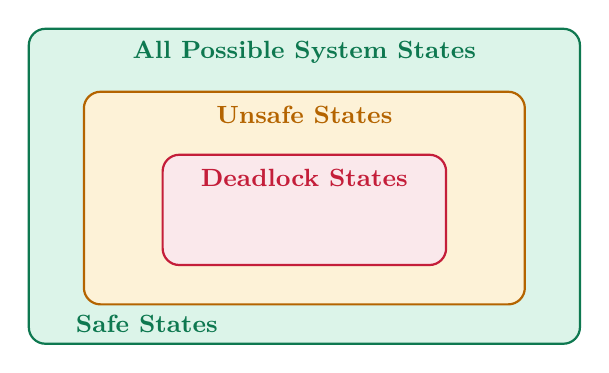
\begin{tikzpicture}[thick, font=\small]
  \draw[draw=mygreen, fill=hdrgreen, rounded corners=6pt] (-3.5, -2.0) rectangle (3.5, 2.0);
  \node[font=\small\bfseries\color{mygreen}] at (0.0, 1.7) {All Possible System States};

  \draw[draw=myamber, fill=hdramber, rounded corners=6pt] (-2.8, -1.5) rectangle (2.8, 1.2);
  \node[font=\small\bfseries\color{myamber}] at (0.0, 0.9) {Unsafe States};

  \draw[draw=myred, fill=hdrred, rounded corners=6pt] (-1.8, -1.0) rectangle (1.8, 0.4);
  \node[font=\small\bfseries\color{myred}] at (0.0, 0.1) {Deadlock States};

  \node[font=\small\bfseries\color{mygreen}] at (-2.0, -1.75) {Safe States};
\end{tikzpicture}
\end{tcolorbox}

\subsubsection{Banker's Algorithm}
Used for systems with multiple instances of resources. Data structures:
\begin{itemize}[leftmargin=*, itemsep=3pt]
  \item \texttt{Available[m]}: Available instances of each resource.
  \item \texttt{Max[n][m]}: Maximum demand of each process.
  \item \texttt{Allocation[n][m]}: Resources currently allocated to each process.
  \item \texttt{Need[n][m]}: Remaining resources a process may request. Note: $\text{Need}[i][j] = \text{Max}[i][j] - \text{Allocation}[i][j]$.
\end{itemize}

\subsection{3. Deadlock Detection \& Recovery}
If a system does not prevent or avoid deadlocks, a deadlock may occur. The OS must provide:
\begin{itemize}[leftmargin=*, itemsep=3pt]
  \item A detection algorithm (periodically runs to find cycles or execute safety checks).
  \item A recovery scheme:
  \begin{itemize}[leftmargin=*, itemsep=2.5pt, topsep=0pt]
    \item \textbf{Process Termination:} Abort all deadlocked processes, or abort one-by-one until the cycle is broken.
    \item \textbf{Resource Preemption:} Preempt resources from some processes, roll back those processes to a safe checkpoint, and restart them.
    \end{itemize}
  \end{itemize}

\newpage
% ===============================================================================
% MANDATORY QUICK REVISION PAGE
% ===============================================================================
\begin{center}
  {\large\bfseries\color{myred} Quick Revision --- Module 5}\\[3pt]
  {\small\color{mydark} Deadlocks $|$ OE-EC604B}
\end{center}
\noindent{\color{myred}\rule{\linewidth}{1.2pt}}
\vspace{4pt}

\begin{tcolorbox}[formulabox, title={\textbf{Banker's Safety Algorithm Equations}}]
Let $\text{Work} = \text{Available}$ and $\text{Finish}[i] = \text{false}$ for $i = 0, 1, \dots, n-1$.
Find an index $i$ such that both:
1. $\text{Finish}[i] == \text{false}$
2. $\text{Need}_i \le \text{Work}$
If such an $i$ exists, update:
$$\text{Work} = \text{Work} + \text{Allocation}_i$$
$$\text{Finish}[i] = \text{true}$$
Repeat. If $\text{Finish}[i] == \text{true}$ for all $i$, the system is in a \textbf{Safe State}.
\end{tcolorbox}

\begin{tcolorbox}[defbox, title={\textbf{One-Line Definitions}}]
\begin{itemize}[leftmargin=*, itemsep=2.5pt, topsep=0pt]
  \item \textbf{Deadlock:} State where processes wait indefinitely for resources held by each other.
  \item \textbf{Mutual Exclusion:} Rule that only one process can hold a resource instance at any time.
  \item \textbf{Hold and Wait:} Process holding resources while requesting more without releasing current ones.
  \item \textbf{Preemption:} Forcible retrieval of allocated resources from a process by the OS.
  \item \textbf{Circular Wait:} Chain of processes where each waits for a resource held by the next.
  \item \textbf{Resource Allocation Graph:} Directed graph showing resource allocations and process requests.
  \item \textbf{Safe Sequence:} Order of process execution that guarantees no deadlock can occur.
  \item \textbf{Ostrich Algorithm:} Deadlock strategy of ignoring the problem (used when deadlocks are rare).
\end{itemize}
\end{tcolorbox}

\begin{tcolorbox}[exambox, title={\textbf{Frequently Asked / Viva Questions}}]
\begin{enumerate}[topsep=0pt, label=\textbf{Q\arabic*.}, itemsep=5pt]
  \item \Q{What are the four necessary conditions for a deadlock to occur?}
    Mutual Exclusion, Hold and Wait, No Preemption, and Circular Wait (Coffman conditions). All four must hold simultaneously for a deadlock to exist.
  \item \Q{Consider a system with 5 processes (P0 to P4) and 3 resource types (A, B, C):}\\
    $\text{Allocation} = \begin{pmatrix} 0 \& 1 \& 0 \\ 2 \& 0 \& 0 \\ 3 \& 0 \& 2 \\ 2 \& 1 \& 1 \\ 0 \& 0 \& 2 \end{pmatrix}, \quad \text{Max} = \begin{pmatrix} 7 \& 5 \& 3 \\ 3 \& 2 \& 2 \\ 9 \& 0 \& 2 \\ 2 \& 2 \& 2 \\ 4 \& 3 \& 3 \end{pmatrix}, \quad \text{Available} = \begin{pmatrix} 3 \& 3 \& 2 \end{pmatrix}$\par
    \textbf{Is the system in a safe state? Find the safe sequence.}\par
    *Step 1: Calculate Need matrix ($\text{Need} = \text{Max} - \text{Allocation}$)*\par
    $\text{Need} = \begin{pmatrix} 7-0 \& 5-1 \& 3-0 \\ 3-2 \& 2-0 \& 2-0 \\ 9-3 \& 0-0 \& 2-2 \\ 2-2 \& 2-1 \& 2-1 \\ 4-0 \& 3-0 \& 3-2 \end{pmatrix} = \begin{pmatrix} 7 \& 4 \& 3 \\ 1 \& 2 \& 2 \\ 6 \& 0 \& 0 \\ 0 \& 1 \& 1 \\ 4 \& 3 \& 1 \end{pmatrix}$\par
    *Step 2: Initialize $\text{Work} = \begin{pmatrix} 3 \& 3 \& 2 \end{pmatrix}$*\par
    \begin{itemize}[leftmargin=*, itemsep=2.5pt, topsep=2pt]
      \item \textbf{Check P1:} $\text{Need}_1 \begin{pmatrix} 1 \& 2 \& 2 \end{pmatrix} \le \text{Work} \begin{pmatrix} 3 \& 3 \& 2 \end{pmatrix}$? Yes. $\text{Work} \to \text{Work} + \text{Alloc}_1 = \begin{pmatrix} 5 \& 3 \& 2 \end{pmatrix}$.
      \item \textbf{Check P3:} $\text{Need}_3 \begin{pmatrix} 0 \& 1 \& 1 \end{pmatrix} \le \text{Work} \begin{pmatrix} 5 \& 3 \& 2 \end{pmatrix}$? Yes. $\text{Work} \to \text{Work} + \text{Alloc}_3 = \begin{pmatrix} 7 \& 4 \& 3 \end{pmatrix}$.
      \item \textbf{Check P0:} $\text{Need}_0 \begin{pmatrix} 7 \& 4 \& 3 \end{pmatrix} \le \text{Work} \begin{pmatrix} 7 \& 4 \& 3 \end{pmatrix}$? Yes. $\text{Work} \to \text{Work} + \text{Alloc}_0 = \begin{pmatrix} 7 \& 5 \& 3 \end{pmatrix}$.
      \item \textbf{Check P2:} $\text{Need}_2 \begin{pmatrix} 6 \& 0 \& 0 \end{pmatrix} \le \text{Work} \begin{pmatrix} 7 \& 5 \& 3 \end{pmatrix}$? Yes. $\text{Work} \to \text{Work} + \text{Alloc}_2 = \begin{pmatrix} 10 \& 5 \& 5 \end{pmatrix}$.
      \item \textbf{Check P4:} $\text{Need}_4 \begin{pmatrix} 4 \& 3 \& 1 \end{pmatrix} \le \text{Work} \begin{pmatrix} 10 \& 5 \& 5 \end{pmatrix}$? Yes. $\text{Work} \to \text{Work} + \text{Alloc}_4 = \begin{pmatrix} 10 \& 5 \& 7 \end{pmatrix}$.
    \end{itemize}
    \textbf{Result:} All processes finished. System is in \textbf{safe state} with safe sequence: $\langle \mathbf{P1, P3, P0, P2, P4} \rangle$.
  \item \Q{Differentiate between Deadlock Prevention and Deadlock Avoidance.}
    Prevention limits system design by enforcing policies that violate one of the 4 Coffman conditions (e.g., resource ordering). Avoidance does not restrict request structures but checks dynamic resource availability and maximum limits to keep the system in a safe state.
  \item \Q{How can the circular wait condition be prevented in operating systems?}
    By defining a global 1-to-1 enumeration function $F: R \to \mathbb{N}$ for all resource types. A process can only request resource $R_j$ if $F(R_j) > F(R_i)$, where $R_i$ is any resource currently held by the process.
  \item \Q{What is an unsafe state? Does it always lead to a deadlock?}
    An unsafe state is a state from which the OS cannot guarantee that all processes can finish their maximum execution. It does \textbf{not} always lead to a deadlock; it will only deadlock if processes actually request their maximum declared resources.
  \item \Q{Why does a cycle in a Resource Allocation Graph (RAG) not always indicate a deadlock?}
    If a resource type has multiple instances, a cycle indicates a potential deadlock but not a guaranteed one, as a process outside the cycle might release an instance, breaking the cycle.
  \item \Q{What is the difference between a Resource Allocation Graph and a Wait-For Graph?}
    A Resource Allocation Graph shows both processes and resources with request/assignment edges. A Wait-For Graph is a simplified version for single-unit resource systems, showing only processes, where edge $P_i \to P_j$ means $P_i$ waits for $P_j$ to release a resource.
  \item \Q{Explain the recovery methods from deadlock.}
    1. Process Termination: Abort all deadlocked processes, or abort processes one-by-one until the cycle is broken. 2. Resource Preemption: Take resources from a process, roll it back to a safe checkpoint, and restart it.
  \item \Q{What is the "Ostrich Algorithm" and when is it appropriate to use?}
    It is the strategy of ignoring deadlocks altogether, assuming they occur rarely. It is used by most general-purpose OS (like Windows/Linux) because deadlock prevention/avoidance adds heavy run-time overhead.
  \item \Q{Why is preemption difficult to implement for some resources?}
    Because some resources (like printers or files being written) cannot be easily saved and restored mid-operation without corrupting data or output.
\end{enumerate}
\end{tcolorbox}

\begin{tcolorbox}[tikzbox, title={Deadlock Handling Trade-offs}]
\renewcommand{\arraystretch}{1.4}
\par\noindent
\begin{tabularx}{\linewidth}{|B{2.2cm}|>{\small\centering\arraybackslash}X|>{\small\centering\arraybackslash}X|>{\small\centering\arraybackslash}X|}
\hline
\textbf{Strategy} & \textbf{\color{myred}Run-time Overhead} & \textbf{\color{myteal}Resource Utilization} & \textbf{\color{myamber}Implementation} \\
\hline
\textbf{Prevention} & None (static rules) & Low (strict limits) & Simple \\
\hline
\textbf{Avoidance} & Moderate (safety checks) & Moderate & Complex (needs max demand) \\
\hline
\textbf{Detection} & High (periodic checks) & High (free allocation) & Moderate \\
\hline
\end{tabularx}
\end{tcolorbox}

\end{document}
